\section{Experiments}
\label{sec:experiments}

\subsection{Datasets}
Open4DHOI~\cite{wen2025efficient} and BEHAVE~\cite{bhatnagar2022behave} datasets are used for our experiments.
Open4DHOI is an open-vocabulary, in-the-wild human-object interaction dataset spanning a wide range of object categories.
From the whole set, we curate a test set of 210 sequences, spanning diverse interactions.
BEHAVE is an indoor interaction dataset that captures the interactions of 8 human subjects and 20 objects in a controlled setting.
We use its official test split, consisting of 340 sequences, for evaluation.


\subsection{Evaluation Metrics}
\label{sec:evaluation_metrics}
For all evaluation, we align the 4D reconstruction to the ground truth (GT) at each frame by translating the human root coordinate to the GT.


\noindent\textbf{Chamfer distance ($\text{CD}_{\text{H}}$, $\text{CD}_{\text{O}}$).}
We measure the Chamfer distance between the reconstructed human and object surfaces and their corresponding GT.
The Chamfer distance is separately computed for the human ($\text{CD}_{\text{H}}$) and object ($\text{CD}_{\text{O}}$) in centimeters.


\noindent\textbf{Contact score ($\text{Contact}$).}
We evaluate contact fidelity by comparing the contact regions of the reconstructed human and object against the GT.
We define the contact map as the human vertices of the SMPL-X mesh surface~\cite{pavlakos2019expressive} within $5~\text{cm}$ of the object surface.
The contact score ($\text{Contact}$) is computed as the harmonic mean of precision and recall between the predicted and GT human contact maps.


\noindent\textbf{Collision ratio ($\text{Collision}$).}
To evaluate physical plausibility, we measure the interpenetration between the reconstructed human and object surfaces.
The collision ratio ($\text{Collision}$) is the percentage of human vertices located within the object mesh.


\noindent\textbf{Acceleration error ($\text{Accel}_{\text{H}}$, $\text{Accel}_{\text{O}}$).}
To evaluate the temporal consistency of the reconstructed 4D motion, we measure the difference between the predicted and GT acceleration.
$\text{Accel}_{\text{H}}$ is computed over the 14 body joints of the SMPL-X model, and $\text{Accel}_{\text{O}}$ is computed over the 3D object center, both reported in centimeters.


\subsection{Ablation Study}
We carry out all ablation studies on Open4DHOI~\cite{wen2025efficient}.


\noindent\textbf{Effectiveness of our optimization process.}


\noindent\textbf{Effectiveness of video decomposition.}
\cref{tab:abl_decomposition} and \cref{fig:abl_decomposition} show the effectiveness of our video decomposition with motion-aware captioning.
The first to third rows evaluate the impact of different text captioning strategies for 4D reconstruction.
Here, standard captioning denotes deriving interaction descriptions without incorporating object motion information, given only the input video.
Using text captions (the second row) produces far more accurate results than reconstructing without captioning (the first row), as text descriptions provide semantic interaction priors that benefit the reconstruction process.
Furthermore, our motion-aware captioning (the third row) better captures dynamic movements by incorporating temporal changes in object motion, leading to more accurate reconstruction.
The third to fifth rows evaluate the effect of video decomposition. % Hmm...
Here, uniform decomposition denotes partitioning the video into fixed 81-frame intervals regardless of interaction state changes.
Without decomposition (the third row), a single global description fails to capture fine-grained interaction details across different sub-actions.
In uniform decomposition (the fourth row), each video segment often contains mixed sub-actions, yielding ambiguous text captions that degrade reconstruction performance.
In contrast, our grounded decomposition (the fifth row) localizes precise sub-action boundaries based on interaction changes, providing clear textual guidance that achieves the best reconstruction results.



\noindent\textbf{Effectiveness of interaction-aware re-rendering.}
\cref{tab:abl_rerendering} and \cref{fig:abl_rerendering} show the impact of our novel-view re-rendering pipeline and its text conditioning strategies.
Without novel-view re-rendering (the first row), reconstructing solely from monocular observations suffers from depth ambiguities, leading to wrong reconstruction.
In contrast, using re-rendering (the second row) provides multi-view supervision to mitigate depth ambiguities.
Furthermore, using our regional text conditioning (the third row) guides the human and the object with separate semantic prompts, ensuring clear boundaries between them in re-rendering.
This provides view-consistent novel-view supervision for the 4D HOI optimization, enabling our framework to accurately reconstruct both the human and the object.

% \noindent\textbf{Ablation on 4D HOI optimization}


\subsection{Comparison with State-of-the-Art Methods}
We compare our framework with state-of-the-art reconstruction methods, categorized with image-based and video-based approaches.
Since the image-based methods optimize each frame independently, evaluating them on the full video is extremely computationally expensive.
We thus compare with the image-based methods on key frames sampled at 1 fps, and report the acceleration error ($\text{Accel}_{\text{H}}$, $\text{Accel}_{\text{O}}$) only for the video-based methods.


\begin{table*}[t]
\def\arraystretch{1.55}
\renewcommand{\tabcolsep}{0.6mm}
\footnotesize

\caption{
    \textbf{Quantitative comparison with state-of-the-art methods on Open4DHOI and BEHAVE.}
    Bold and underlined values indicate the best and second-best scores, respectively.
}
\label{tab:sota_comparison}

\vspace*{-0.2em}
\begin{center}
\scalebox{0.68}{
    \begin{tabular}{
    >{\centering\arraybackslash}m{0.4cm}
    >{\raggedright\arraybackslash}m{2.65cm}|
    >{\centering\arraybackslash}m{1.2cm}
    >{\centering\arraybackslash}m{1.2cm}
    >{\centering\arraybackslash}m{1.35cm}
    >{\centering\arraybackslash}m{1.5cm}
    >{\centering\arraybackslash}m{1.3cm}
    >{\centering\arraybackslash}m{1.3cm}|
    >{\centering\arraybackslash}m{1.2cm}
    >{\centering\arraybackslash}m{1.2cm}
    >{\centering\arraybackslash}m{1.35cm}
    >{\centering\arraybackslash}m{1.5cm}
    >{\centering\arraybackslash}m{1.3cm}
    >{\centering\arraybackslash}m{1.3cm}
    }
    \specialrule{.1em}{.05em}{0.0em}

        \multicolumn{2}{l|}{}
        & \multicolumn{6}{c|}{Open4DHOI}
        & \multicolumn{6}{c}{BEHAVE} \\

        \multicolumn{2}{l|}{Methods}
        & $\text{CD}_{\text{H}}{\downarrow}$
        & $\text{CD}_{\text{O}}{\downarrow}$
        & $\text{Contact}{\uparrow}$
        & $\text{Collision}{\downarrow}$
        & $\text{Accel}_{\text{H}}{\downarrow}$
        & $\text{Accel}_{\text{O}}{\downarrow}$
        & $\text{CD}_{\text{H}}{\downarrow}$
        & $\text{CD}_{\text{O}}{\downarrow}$
        & $\text{Contact}{\uparrow}$
        & $\text{Collision}{\downarrow}$
        & $\text{Accel}_{\text{H}}{\downarrow}$
        & $\text{Accel}_{\text{O}}{\downarrow}$ \\
        \hline

        \multirow{4}{*}{\rotatebox{90}{Image-based\;\;}}
        & PHOSA
        & 6.434 & 61.138 & 0.267 & \underline{0.061} & -- & --
        & 5.661 & 40.355 & 0.326 & 0.099 & -- & -- \\

        & HOI-Gaussian
        & \textbf{5.330} & 47.086 & 0.382 & 0.072 & -- & --
        & \textbf{3.420} & 39.722 & 0.521 & \underline{0.097} & -- & -- \\

        & TeHOR
        & 5.501 & \underline{44.397} & \underline{0.456} & 0.070 & -- & --
        & 3.627 & \underline{31.168} & \underline{0.552} & 0.099 & -- & -- \\

        & \textbf{\ourmethod~(Ours)}
        & \underline{5.380} & \textbf{37.268} & \textbf{0.501} & \textbf{0.056} & -- & --
        & \underline{3.512} & \textbf{13.013} & \textbf{0.569} & \textbf{0.080} & -- & -- \\

        \hline

        \multirow{4}{*}{\rotatebox{90}{Video-based\;\;}}
        & VisTracker
        & 6.392 & 51.289 & 0.383 & \underline{0.152} & \underline{0.459} & \underline{2.197}
        & 6.049 & 16.664 & 0.464 & \underline{0.108} & 1.553 & 1.336 \\

        & InterTrack
        & 7.143 & 49.110 & 0.482 & 0.218 & 2.534 & 5.996
        & 9.487 & 19.441 & 0.560 & 0.268 & 2.258 & 5.427 \\

        & CARI4D
        & \underline{5.740} & \underline{39.090} & \underline{0.514} & 0.182 & 0.710 & 2.332
        & \underline{3.582} & \underline{14.213} & \underline{0.583} & 0.130 & \underline{0.990} & \underline{1.148} \\

        & \textbf{\ourmethod~(Ours)}
        & \textbf{5.385} & \textbf{34.894} & \textbf{0.520} & \textbf{0.056} & \textbf{0.273} & \textbf{1.571}
        & \textbf{3.341} & \textbf{12.932} & \textbf{0.592} & \textbf{0.075} & \textbf{0.312} & \textbf{0.981} \\

        \specialrule{.1em}{-0.05em}{-0.05em}
    \end{tabular}
}
\end{center}
\vspace*{-1.2em}
\end{table*}
\begin{figure*}[t!]
  \centering
  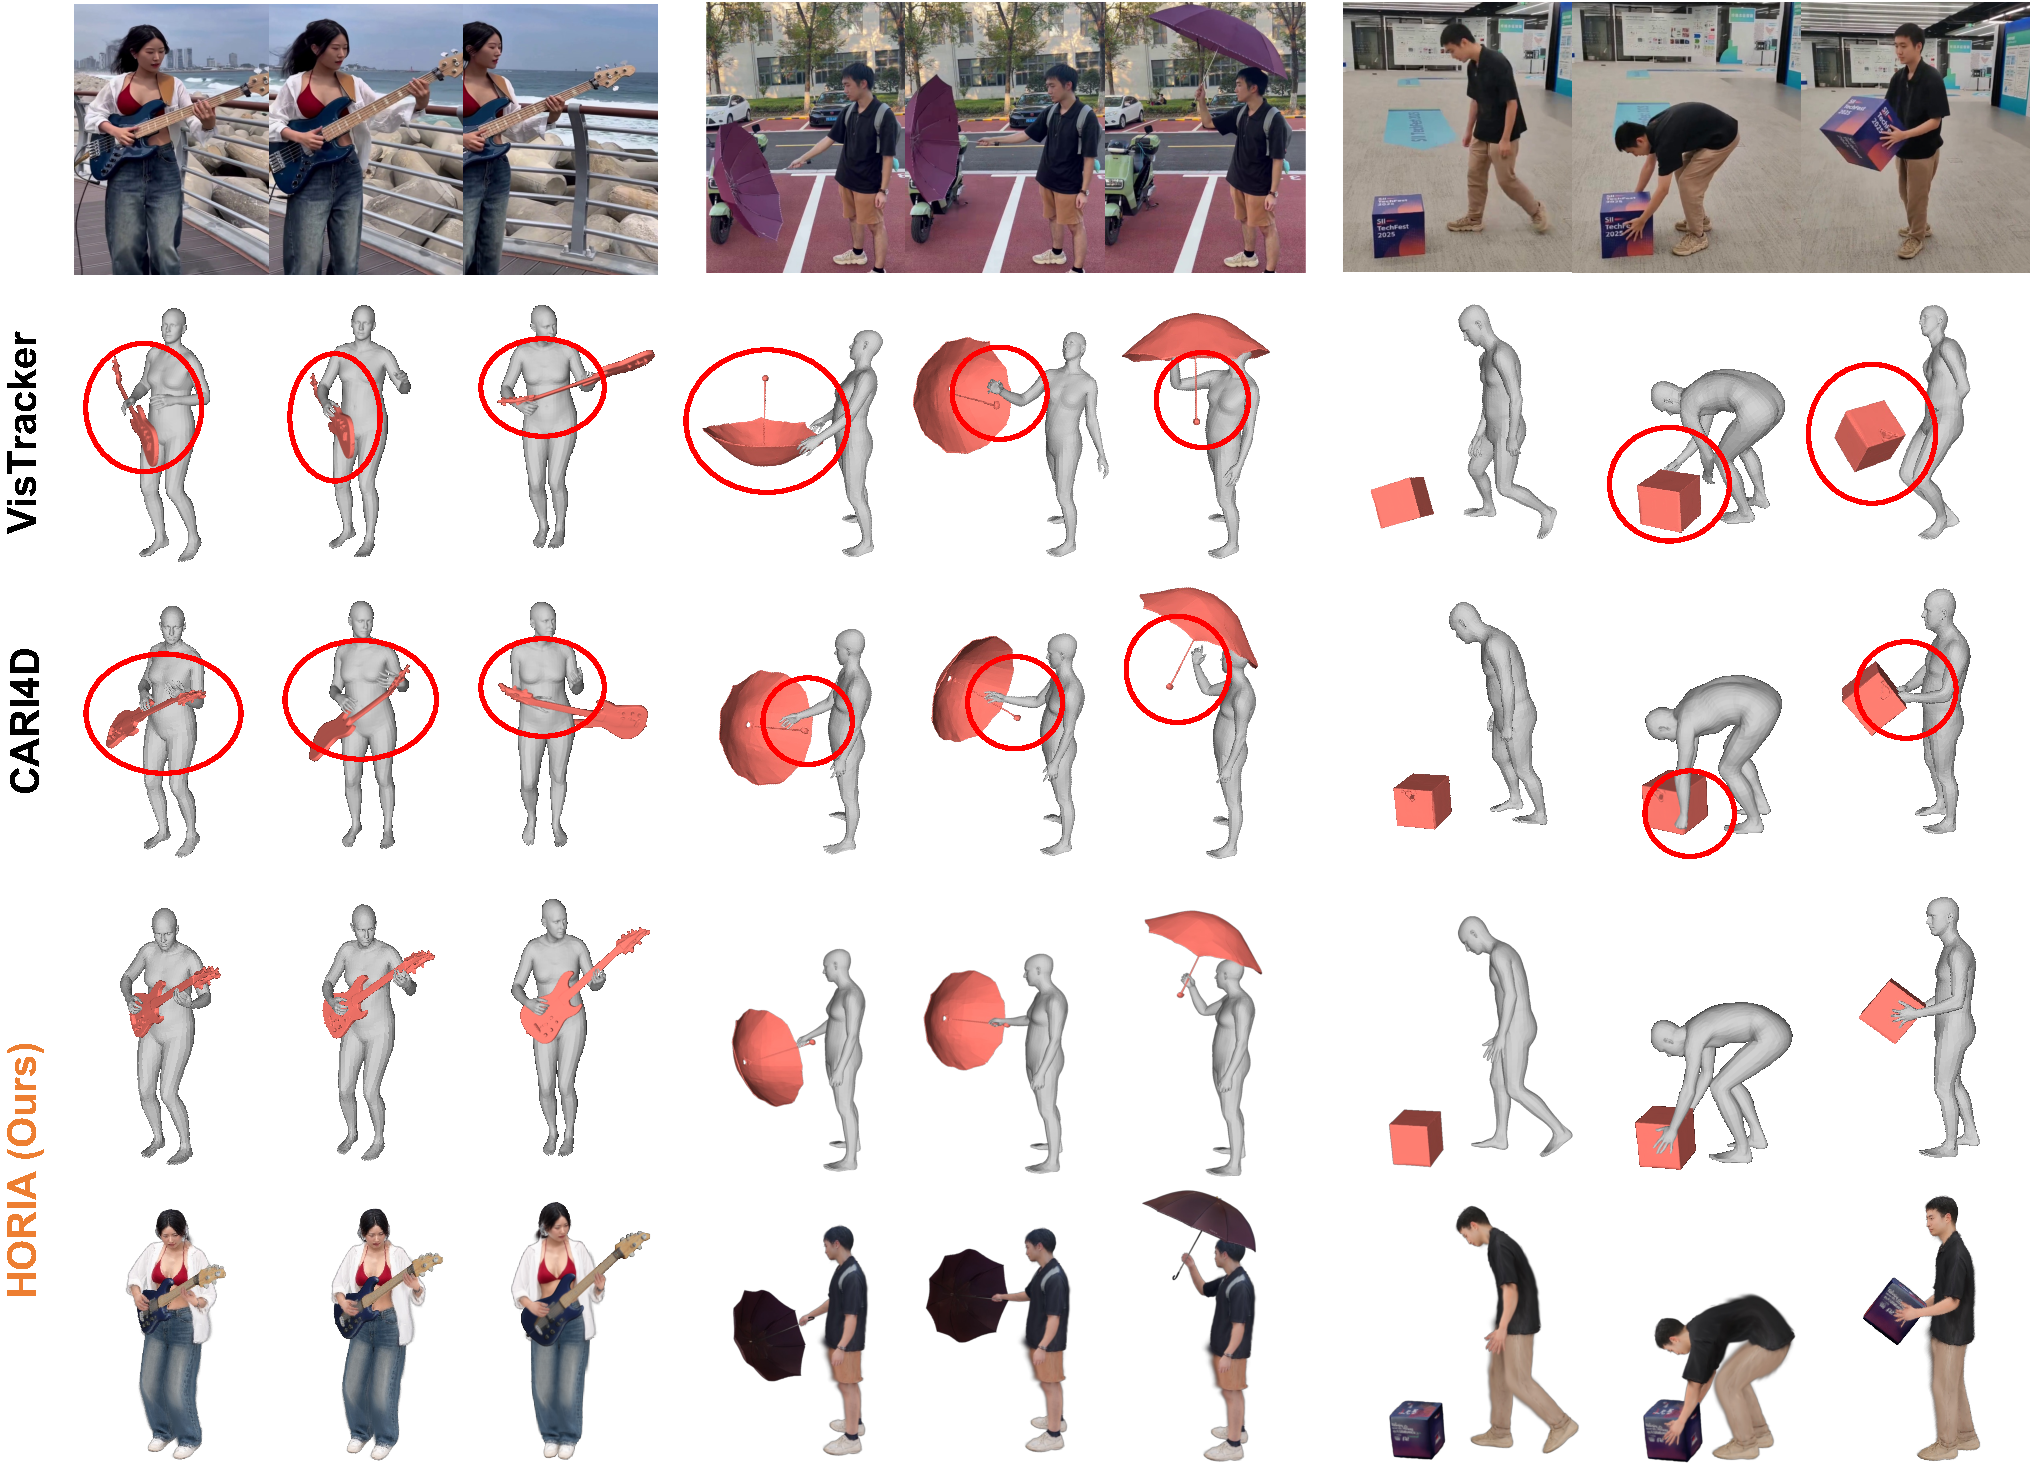
\includegraphics[width=1.0\linewidth]{figures/6_sota_comparison.pdf}
  \vspace*{-1.5em}
  \caption{\textbf{Qualitative comparison with state-of-the-art methods.}
  We render each method's reconstruction at $+30^\circ$ azimuth and highlight representative failure cases with red circles.
  }
   \vspace*{+0.0em}
  \label{fig:6_sota_comparison}
\end{figure*}


\cref{fig:6_sota_comparison} and \cref{tab:sota_comparison} show that \ourmethod~outperforms all baselines both qualitatively and quantitatively on Open4DHOI and BEHAVE.
As shown in \cref{fig:6_sota_comparison}, VisTracker and CARI4D frequently misplace the object relative to the hand or body during close interaction, since both methods reason about human-object poses primarily from geometric and contact cues without semantic understanding of the interaction.
InterTrack reconstructs the human and object as noisy point clouds without a consistent surface, which further degrades reconstruction accuracy under occlusion.
Among image-based methods, HOI-Gaussian leverages depth information as an additional prior, but remains vulnerable to severe human-object occlusion and cannot capture the semantic context of the interaction.
Unlike these methods, \ourmethod~leverages temporally grounded text descriptions of each sub-action, providing semantic context that geometric and contact cues alone cannot capture, and further enforces cross-view geometric consistency via the SDF loss, achieving the lowest collision ratio and acceleration error among all baselines.
